
%% bare_conf.tex
%% V1.3
%% 2007/01/11
%% by Michael Shell
%% See:
%% http://www.michaelshell.org/
%% for current contact information.
%%
%% This is a skeleton file demonstrating the use of IEEEtran.cls
%% (requires IEEEtran.cls version 1.7 or later) with an IEEE conference paper.
%%
%% Support sites:
%% http://www.michaelshell.org/tex/ieeetran/
%% http://www.ctan.org/tex-archive/macros/latex/contrib/IEEEtran/
%% and
%% http://www.ieee.org/

%%*************************************************************************
%% Legal Notice:
%% This code is offered as-is without any warranty either expressed or
%% implied; without even the implied warranty of MERCHANTABILITY or
%% FITNESS FOR A PARTICULAR PURPOSE!
%% User assumes all risk.
%% In no event shall IEEE or any contributor to this code be liable for
%% any damages or losses, including, but not limited to, incidental,
%% consequential, or any other damages, resulting from the use or misuse
%% of any information contained here.
%%
%% All comments are the opinions of their respective authors and are not
%% necessarily endorsed by the IEEE.
%%
%% This work is distributed under the LaTeX Project Public License (LPPL)
%% ( http://www.latex-project.org/ ) version 1.3, and may be freely used,
%% distributed and modified. A copy of the LPPL, version 1.3, is included
%% in the base LaTeX documentation of all distributions of LaTeX released
%% 2003/12/01 or later.
%% Retain all contribution notices and credits.
%% ** Modified files should be clearly indicated as such, including  **
%% ** renaming them and changing author support contact information. **
%%
%% File list of work: IEEEtran.cls, IEEEtran_HOWTO.pdf, bare_adv.tex,
%%                    bare_conf.tex, bare_jrnl.tex, bare_jrnl_compsoc.tex
%%*************************************************************************

% *** Authors should verify (and, if needed, correct) their LaTeX system  ***
% *** with the testflow diagnostic prior to trusting their LaTeX platform ***
% *** with production work. IEEE's font choices can trigger bugs that do  ***
% *** not appear when using other class files.                            ***
% The testflow support page is at:
% http://www.michaelshell.org/tex/testflow/



% Note that the a4paper option is mainly intended so that authors in
% countries using A4 can easily print to A4 and see how their papers will
% look in print - the typesetting of the document will not typically be
% affected with changes in paper size (but the bottom and side margins will).
% Use the testflow package mentioned above to verify correct handling of
% both paper sizes by the user's LaTeX system.
%
% Also note that the "draftcls" or "draftclsnofoot", not "draft", option
% should be used if it is desired that the figures are to be displayed in
% draft mode.
%
\documentclass[10pt, conference, compsocconf]{IEEEtran}
% Add the compsocconf option for Computer Society conferences.
%
% If IEEEtran.cls has not been installed into the LaTeX system files,
% manually specify the path to it like:
% \documentclass[conference]{../sty/IEEEtran}





% Some very useful LaTeX packages include:
% (uncomment the ones you want to load)


% *** MISC UTILITY PACKAGES ***
%
%\usepackage{ifpdf}
% Heiko Oberdiek's ifpdf.sty is very useful if you need conditional
% compilation based on whether the output is pdf or dvi.
% usage:
% \ifpdf
%   % pdf code
% \else
%   % dvi code
% \fi
% The latest version of ifpdf.sty can be obtained from:
% http://www.ctan.org/tex-archive/macros/latex/contrib/oberdiek/
% Also, note that IEEEtran.cls V1.7 and later provides a builtin
% \ifCLASSINFOpdf conditional that works the same way.
% When switching from latex to pdflatex and vice-versa, the compiler may
% have to be run twice to clear warning/error messages.






% *** CITATION PACKAGES ***
%
%\usepackage{cite}
% cite.sty was written by Donald Arseneau
% V1.6 and later of IEEEtran pre-defines the format of the cite.sty package
% \cite{} output to follow that of IEEE. Loading the cite package will
% result in citation numbers being automatically sorted and properly
% "compressed/ranged". e.g., [1], [9], [2], [7], [5], [6] without using
% cite.sty will become [1], [2], [5]--[7], [9] using cite.sty. cite.sty's
% \cite will automatically add leading space, if needed. Use cite.sty's
% noadjust option (cite.sty V3.8 and later) if you want to turn this off.
% cite.sty is already installed on most LaTeX systems. Be sure and use
% version 4.0 (2003-05-27) and later if using hyperref.sty. cite.sty does
% not currently provide for hyperlinked citations.
% The latest version can be obtained at:
% http://www.ctan.org/tex-archive/macros/latex/contrib/cite/
% The documentation is contained in the cite.sty file itself.






% *** GRAPHICS RELATED PACKAGES ***
%
\ifCLASSINFOpdf
  % \usepackage[pdftex]{graphicx}
  % declare the path(s) where your graphic files are
  % \graphicspath{{../pdf/}{../jpeg/}}
  % and their extensions so you won't have to specify these with
  % every instance of \includegraphics
  % \DeclareGraphicsExtensions{.pdf,.jpeg,.png}
\else
  % or other class option (dvipsone, dvipdf, if not using dvips). graphicx
  % will default to the driver specified in the system graphics.cfg if no
  % driver is specified.
  % \usepackage[dvips]{graphicx}
  % declare the path(s) where your graphic files are
  % \graphicspath{{../eps/}}
  % and their extensions so you won't have to specify these with
  % every instance of \includegraphics
  % \DeclareGraphicsExtensions{.eps}
\fi
% graphicx was written by David Carlisle and Sebastian Rahtz. It is
% required if you want graphics, photos, etc. graphicx.sty is already
% installed on most LaTeX systems. The latest version and documentation can
% be obtained at:
% http://www.ctan.org/tex-archive/macros/latex/required/graphics/
% Another good source of documentation is "Using Imported Graphics in
% LaTeX2e" by Keith Reckdahl which can be found as epslatex.ps or
% epslatex.pdf at: http://www.ctan.org/tex-archive/info/
%
% latex, and pdflatex in dvi mode, support graphics in encapsulated
% postscript (.eps) format. pdflatex in pdf mode supports graphics
% in .pdf, .jpeg, .png and .mps (metapost) formats. Users should ensure
% that all non-photo figures use a vector format (.eps, .pdf, .mps) and
% not a bitmapped formats (.jpeg, .png). IEEE frowns on bitmapped formats
% which can result in "jaggedy"/blurry rendering of lines and letters as
% well as large increases in file sizes.
%
% You can find documentation about the pdfTeX application at:
% http://www.tug.org/applications/pdftex





% *** MATH PACKAGES ***
%

\usepackage[cmex10]{amsmath}
\usepackage{tikz}

\definecolor{bluekeywords}{rgb}{0,0,1}
\definecolor{greencomments}{rgb}{0,0.5,0}
\definecolor{redstrings}{rgb}{0.64,0.08,0.08}
\definecolor{xmlcomments}{rgb}{0.5,0.5,0.5}
\definecolor{types}{rgb}{0.17,0.57,0.68}

\usepackage{listings}
\lstset{language=[Sharp]C,
captionpos=b,
numbers=left, %Nummerierung
numberstyle=\tiny, % kleine Zeilennummern
frame=lines, % Oberhalb und unterhalb des Listings ist eine Linie
showspaces=false,
showtabs=false,
breaklines=true,
showstringspaces=false,
breakatwhitespace=true,
escapeinside={(*@}{@*)},
commentstyle=\color{greencomments},
morekeywords={partial, var, value, get, set},
keywordstyle=\color{bluekeywords},
stringstyle=\color{redstrings},
basicstyle=\scriptsize,
}

\usepackage[]{algorithm}
\usepackage{algorithmic}
\usepackage{etoolbox}
\usepackage{subfig}


\newcommand{\algorithmicdoinparallel}{\textbf{do in parallel}}
\makeatletter
\AtBeginEnvironment{algorithmic}{%
  \newcommand{\FORALLP}[2][default]{\ALC@it\algorithmicforall\ #2\ %
    \algorithmicdoinparallel\ALC@com{#1}\begin{ALC@for}}%
}
\makeatother


% correct bad hyphenation here
\hyphenation{op-tical net-works semi-conduc-tor}

\newtheorem{theorem}{Theorem}[section]
\newtheorem{lemma}[theorem]{Lemma}
\newtheorem{proposition}[theorem]{Proposition}
\newtheorem{corollary}[theorem]{Corollary}
\newtheorem{property}[theorem]{Property}
\newtheorem{definition}[theorem]{Definition}
\newtheorem{remark}[theorem]{Remark}
\newtheorem{assumption}[theorem]{Assumption}

\newcommand{\norm}[1]{\left\lVert#1\right\rVert}


\begin{document}
%
% paper title
% can use linebreaks \\ within to get better formatting as desired
\title{Acoustic fall detection with Bootstrap Aggregating classifiers}


% author names and affiliations
% use a multiple column layout for up to two different
% affiliations

\author{\IEEEauthorblockN{Loukas Kominis}
\IEEEauthorblockA{
Department of ECE, \\
University of Patras,\\
 Patras, Greece\\
loukaskom@gmail.com}
\and
\IEEEauthorblockN{Yanik Ngoko}
\IEEEauthorblockA{Qarnot computing and University of Paris 13\\
Montrouge, France\\
yanik.ngoko@qarnot-computing.com}
\and
\IEEEauthorblockN{Christophe C\'erin}
\IEEEauthorblockA{University of Paris 13\\
Paris, France\\
christophe.cerin@lipn.univ-paris13.fr}

}

%\author{\IEEEauthorblockN{Yanik Ngoko}
%\IEEEauthorblockA{Qarnot Computing and University of Paris 13\\
%Paris, France\\
%yanik.ngoko@\{qarnot-computing.com, lipn.univ-paris13.fr\}}
%\and
%\IEEEauthorblockN{Christophe C\'erin}
%\IEEEauthorblockA{University of Paris 13\\
%Paris, France\\
%christophe.cerin@lipn.univ-paris13.fr}
%}


% conference papers do not typically use \thanks and this command
% is locked out in conference mode. If really needed, such as for
% the acknowledgment of grants, issue a \IEEEoverridecommandlockouts
% after \documentclass

% for over three affiliations, or if they all won't fit within the width
% of the page, use this alternative format:
%
%\author{\IEEEauthorblockN{Michael Shell\IEEEauthorrefmark{1},
%Homer Simpson\IEEEauthorrefmark{2},
%James Kirk\IEEEauthorrefmark{3},
%Montgomery Scott\IEEEauthorrefmark{3} and
%Eldon Tyrell\IEEEauthorrefmark{4}}
%\IEEEauthorblockA{\IEEEauthorrefmark{1}School of Electrical and Computer Engineering\\
%Georgia Institute of Technology,
%Atlanta, Georgia 30332--0250\\ Email: see http://www.michaelshell.org/contact.html}
%\IEEEauthorblockA{\IEEEauthorrefmark{2}Twentieth Century Fox, Springfield, USA\\
%Email: homer@thesimpsons.com}
%\IEEEauthorblockA{\IEEEauthorrefmark{3}Starfleet Academy, San Francisco, California 96678-2391\\
%Telephone: (800) 555--1212, Fax: (888) 555--1212}
%\IEEEauthorblockA{\IEEEauthorrefmark{4}Tyrell Inc., 123 Replicant Street, Los Angeles, California 90210--4321}}




% use for special paper notices
%\IEEEspecialpapernotice{(Invited Paper)}




% make the title area
\maketitle


\begin{abstract}

We consider the design of an acoustic fall detection system with the Qarnot model of computing. 
Qarnot introduced a computing model based on heaters that embed several processors and sensors. 
The network of Qarnot heaters in a home and building offers several advantages for the design of smart-environments 
systems when we consider the privacy, the real-life performance or the acceptance. 
The main goal of this work is to show the effectiveness of this platform for the resolution of smart-home problems  
and acoustic fall detection in particular. 
In addition to consider the Qarnot context, our work also innovates in applying bootstrap aggregation on  
acoustic fall detection. The results we obtained are very encouraging. We were able to build a classifier 
whose accuracy is higher than what we found in the state of the art on the problem. Moreover, though the results were obtained in 
using Qarnot tools for the design of smart-environment systems, they can be generalized to other contexts.
\end{abstract}

\begin{IEEEkeywords}
acoustic fall detection; smart-environment; bootstrap aggregation

\end{IEEEkeywords}


% For peer review papers, you can put extra information on the cover
% page as needed:
% \ifCLASSOPTIONpeerreview
% \begin{center} \bfseries EDICS Category: 3-BBND \end{center}
% \fi
%
% For peerreview papers, this IEEEtran command inserts a page break and
% creates the second title. It will be ignored for other modes.
\IEEEpeerreviewmaketitle


\section{Introduction}
\label{introduction}

The demographic explosion of the eldery is offering and unprecendented opportunity for the development of a
assisted living technologies. However, the question of the right architecture for such technologies is critical. 
By the past, several concerns were raised on existing solutions. The sensitive topics include the privacy, 
the acceptance or the real-life performance of such technologies. For the interested reader, we recommend the work of 
 Igual et al.~\cite{Igual2013}. 

In this paper, we focus on the design of a fall detection system for elders. The conviction that supports our work is 
that with the Qarnot model of computing~\footnote{www.qarnot-computing.com}, we can design a fall detection system 
where several of the  classical concerns regarding assisted living technologies are addressed. Qarnot introduced 
a utility computing model where the computing nodes are heaters that are embedded in homes, offices, buildings where they serve 
to heat. These special computing nodes (called Q.rads) embed several processors but also sensors related for instance to 
humidity, $\mathrm{CO_2}$, noise, presence etc. The heaters are connected to the Internet and at the upper level, the network 
of geo-distributed Q.rads is exploited as an HPC cloud infrastructure (See Figure~\ref{fig:digital}). At the scale of homes 
and buildings in which the Q.rads are deployed, this network serves as a smart-building platform with some services like 
the analysis of the air quality or the detection of the sounds of fire-alarms. For more details about the Qarnot model, 
we refer the interested reader to~\cite{DBLP:conf/europar/Ngoko16}.

	\begin{figure*}[htbp]
	\subfloat[{\scriptsize A Q.rad}]{
            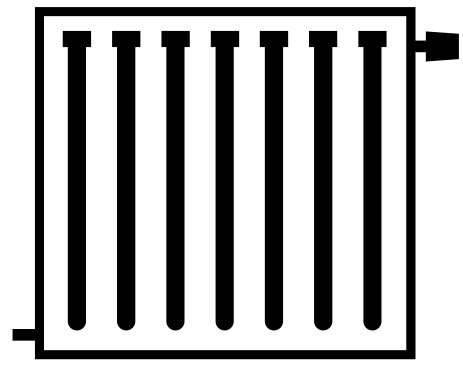
\includegraphics[width=4cm,height=3.5cm]{./Figures/rad.png}
         }
	\subfloat[{\scriptsize The Qarnot model for HPC-cloud}]{
            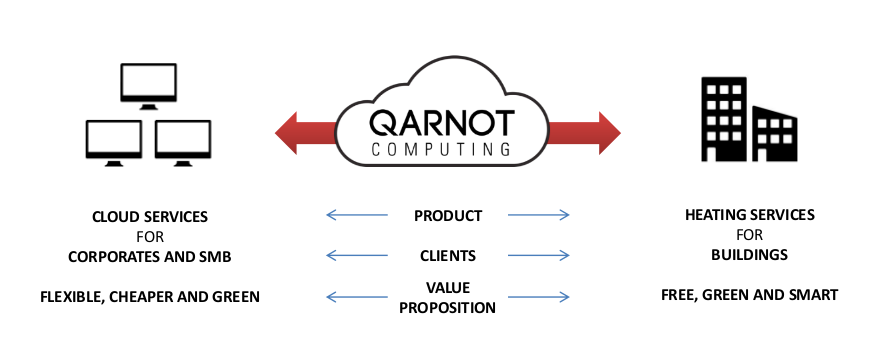
\includegraphics[width=10.7cm,height=3.5cm]{./Figures/model.png}
        }
	\caption{The Qarnot model}
	\label{fig:digital}
	\end{figure*}

In the Qarnot vision, the process view of a smart-environment (home or building) consists of a forest of distributed 
worflows that are locally orchestrated in the Q.rads to which the environment belongs. Here, the data used by the processes are 
issued from the sensors embedded in Q.rads or remotely. A process could for instance analyze the level of $\mathrm{CO_2}$ to make 
recommendations on the need to open windows. Another process could continuously analyze the sound flow that are collected 
at the level of Q.rads in order to see whether or not there is a fall. 
Regarding data privacy, in this vision, we can guarantee that all data collected in a building will remain in the building. 
This changes from classical cloud-based smart-homes where the data are saved remotely in a datacenter. 
Regarding acceptance by elders, the Qarnot solution does not require any wearable device, nor a smartphone to collect user data. 
The user does not even need to care about the functioning of their heater. Finally for real-life performance, because of the sensing and 
computing power of the heaters~\footnote{ A heater could embed $4$ processors}, we have enough computing power to locally 
calibrate a machine learning model, for the specific environment in which we operate.
In this paper, we will present the results we got on a distributed training system (machine learning system), 
we designed in order to detect falls with the Qarnot model of computing. 

The automatic fall detection is an old smart-home topic. Several machine learning systems were already 
proposed for its resolution. A good survey on the diverse contributions can be found in~\cite{Igual2013,Mubashir:2013:SFD:2397722.2397898}. 
Despite the interest and quality of these solutions, our work has some specificities that were not addressed in past 
works. Indeed, past systems were often based on videos, accelerometers or smart-phones while we are mainly based on 
acoustic data. The choice to consider acoustic inputs comes from the fact that the Qarnot heaters do not embed cameras. In addition, 
we consider that the solution of an accelerometer or a smart-phone is not efficient in the viewpoint of the acceptance or 
usability by the elders. 

Acoustic fall detection systems were considered in the past. For instance, we can refer to the work of Xiaodan Zhuang~\cite{Xiaodan2009} where GMM and SVM classifier were used and they managed to achieve a fall accuracy of 59\% and 67\% respectively with using only a far-field microphone. Other insteresting works on this field are the ones of Yun~\cite{Yun2012} and Muhammad~\cite{Muhammad2014} that use audio data to achieve classification of falls, each of them in a specific way.  

Differently to these works, we innovate in two points. The first is that we designed a training system to run on 
the Qarnot cloud. This was achieved in using the Software Defined Kit of Qarnot to build a solution that is orchestrated by 
the Q.ware resoyrce manager. The second point is that differently from existing works, we used the  bootstrap aggregation. 

Bootstrap aggregating, also known as bagging, is a machine learning ensemble meta-algorithm which was designed to improve the stability and accuracy of machine learning algorithms by combining classifications of randomly generated training sets. Bagging can reduce variance and help to avoid the problem of overfitting. Usually it is applied to decision tree methods, but it can be applied to any method. The usage of this techniques leads to an important finding: we were able to build a meta-classifier, 
largely more accurate than all the other classifiers taken separately. We even obtained accuracy and True positive scores that 
we did not find in the literature. 

The remainder of this paper is organized as follows. In Section~\ref{Related}, we present the related works. Section~\ref{Smart} 
present Qarnot tools for smart environments. We detail here the architectural context in which we want to develop a fall 
detection system. Section~\ref{Fall} discusses of the training of a fall detection system with three classifiers: SVM, KNN and decision tree. 
In Section~\ref{BaggingFall} we reconsider the question with Bagging. In Section~\ref{Conclusion}, we conclude.

\section{Related Works} \label{Related}

{\bf TODO}

\section{Qarnot tools for smart environments} \label{Smart}

{\bf To add info for QaIoT, Q.ware etc}


\section{Building fall detection classifiers} \label{Fall}

\subsection{Creating the Dataset} 
 
In order to be able to design an accurate system, it is really important to create a dataset of significant quality. As for a system like this, it is not easy to create a dataset from the very beginning, we used as main source an already existing Laboratory research dataset~\cite{Dataset}. It contained video data which consisted of falls and other no-fall activities in different environments and especially Office, Home, Coffee room and Lecture room. The frame rate is 25 frames/s and the resolution 320x240 pixels. The dataset containes 191 videos of different time durations, from 6 sec to 1.20 minutes. The use of different environments makes the dataset more complete and representative in compare to others.  

\subsubsection{Audio Extraction}

Using the Audacity software, we extracted the audio and isolated the fall and no-fall segments. The duration of all extracted segments is 5 seconds. Also a re-sampling was done to the audio files in order to have the same sampling rate (44100 Hz) in all of them and they were also converted to monophonic so that they can be used by our python code and libraries used.

\subsubsection{Noise Mixing and Features extraction}

Next step of the procedure was the audio files to get mixed with different types of noise (in all available combinations), so that our dataset is an accurate representation of real-life everyday sounds. At the end, the dataset consists of two major categories, Falls and No-falls, each of them containing a big variety of samples from all the different environments that were used to record the videos. So it is clear that our dataset in now complete. After finishing with the creation of the dataset, next step is to extract the features needed to run the algorithms. For this purpose, an open source library was used, the pyAudioAnalysis python library~\cite{giannakopoulos2015pyaudioanalysis} which extracts specific features for each audio file. These features will be used to train the machine learning algorithms.

\subsubsection{Subsets creation}

The last step to the dataset creation, is to split it in Training and Testing subsets. The proportion remains constant for the entire duration of this experimental research project. Training subset includes 80\% of the main dataset samples and Testing subset 20\%. This split is required in order to produce learning curves for each classifier and also have cross-validation during training them.

\subsection{SVM and kNN implementation}

After our dataset was fully complete and ready to use in training, SVM and kNN classifiers were implemented on it. In part we present the work done in four experimentation Phases, where the algorithms run in different proportions of data and cover all possible scenarios. The proportion of falls and no falls will be increased and decreased respectively in each Phase in order to check how the algorithms respond on the amount of data given.

The Scikit-Learn python library is used for importing the code, needed for the classifiers, to our main python code. Scikit-Learn library was selected as it provides an easy, universal way for importing different classifiers. 

In each classifier used, after training is finished, which is done using the Q.ware platform and actual Q.rads as computing nodes, the five most efficient classifiers are selected and a choice of the best one is made, among them, based on shortest training time. Because apart from the scores and high accuracy we try to accomplish, a time-efficient method is also important to be created. The most important part is the evaluation of the classifier, where the best classifier is used on both Testing and Training Dataset and see through the Learning Curves and the scores of the confusion matrix, which are presented, how the classifier responds as the amount of data is increasing. 

\subsubsection{Phases workflow and results}

In total our experimental section consists of four Phases. In each of them, a different proportion of fall and no fall data was used in order to check the response of the algorithms. In Table 1, the proportions and total amount of data are presented for each Phase. 

In Phase 1, only SVM classifier is trained and we chose to begin with this specific one as it is mostly used to other researches. The results though were definitely not what we expected as at first True-positive rate is really low and False-positive rate seemed unrealistic as a value. The duration of audio data in this phase (audio segment of fall or no fall mixed with noise) was 10 seconds and proportion of falls and no falls was 20-80\%. 

In Phase 2, it was decided to reduce duration of the audio data to 5 seconds in order to make it easier for the classifier to detect the fall part. It would also improve training time. Falls and no falls proportion was 40-60\%. Also the KNN classifier was introduced and trained for the first try as an effort to compare results with SVM. Better results were produced to the SVM, as the True-positive rate increased by 20\%. KNN had similar scores to the SVM as shown in the table, but in general these results are not yet acceptable in order for our system to be independent. 

So moving on to Phase 3, SVM and KNN classifiers were trained again, duration of audio data is still 5 seconds and proportion of data is changed to 50-50\% and we hoped to improve more the scores of the classifiers. But instead of our expectations for continuous improvement, the SVM results were dissapointing. Not only scores did not icrease but they deteriorated. KNN on the other hand, had better results. This difference in the results can be explained by the different definition of the two classifiers. As KNN detects similarities in a close nearby area it is profited by adding more fall data. In this phase, it was when we first thought of having a different approach on the way of classification, as the system seems to have a kind of sensitivity to the amount of data given each time, that it is not easy to regulate. 

As it was needed to see if our thoughts had logical basis, we moved on to Phase 4. Here, the same settings are used, except the proportion of data used, which changed to 60-40\% of falls and no falls. And the results, certified our theory of sensitivity. The SVM classifier, had a significant improvement and for sure these were the best scores achieved with this specific classifier. KNN still produced good results but not with such a huge improvement to its scores. 

By checking the results shown in Table 2, which presents the scores of each classifier for all four experimentation Phases, the above described are more clear. Three are the categories presented. False-positive-rate (F.P.R), True-positive-rate (T.P.R) and Accuracy.  

\begin{table}[ht]
\caption{\it Proportions of data, for each Phase}
\label{Proportions}
\begin{center}
\begin{small}
\begin{sc}
\begin{tabular}{|l|c|c|c|r|}
\hline
Phase & Fall & Fall(\%) & No Fall & No Fall(\%) \\
      & Samples &        & Samples &            \\ 
\hline
1    & 1600 & 20 & 4800 & 80 \\
\hline
2    & 2400 & 40 & 4000 & 60 \\
\hline
3    & 3200 & 50 & 3200 & 50 \\
\hline
4    & 4000 & 60 & 2400 & 40 \\
\hline
\end{tabular}
\end{sc}
\end{small}
\end{center}
\vskip 0.1in
\end{table}

\begin{table}[t]
\caption{\it Classifiers scores, in each Phase}
\label{Scores}
\vskip 0.1in
\begin{center}
\begin{small}
\begin{sc}
\begin{tabular}{|l|c|c|c|r|}
\hline
Phase & Classifier & F.P.R & T.P.R & Accuracy\\
\hline
Ph.1    & SVM & 0.00 & 0.18 & 0.79 \\
\hline
Ph.2    & SVM & 0.12 & 0.45 & 0.75 \\
     & KNN & 0.10 & 0.42 & 0.73 \\
\hline
Ph.3    & SVM & 0.40 & 0.20 & 0.40 \\
	 & KNN & 0.17 & 0.78 & 0.80 \\
\hline
Ph.4    & SVM & 0.20 & 0.92 & 0.90 \\
	 & KNN & 0.21 & 0.79 & 0.77 \\
\hline
\end{tabular}
\end{sc}
\end{small}
\end{center}
\vskip -0.3in
\end{table}

\subsection{Figures}

Here we present the learning curves for each of the four experimental Phases previously described in order to visualize our results. 



\subsection{Conclusion}

After testing SVM and KNN classifiers in different amount of data and comparing their scores, it is clear that this kind of system behaves differently depending on the amount of data given each time. The SVM results leave no doubt to this statement. KNN has better scores, but as explained previously it is due to the way it works and classifies falls. Our main accomplishment is the one presented on next section.

\section{Fall detection with bagging} \label{BaggingFall}
 

The results of the previous experimentations, made us considering a different approach for this type of system. The data sensitivity issue had to be solved. So in this Section, a new classifier is introduced in order to help us achieve better scores and easier classification of falls and solve the data sensitivity issue. Bootstrap Aggregating, commonly known as Bagging, is an ensemble meta-estimator. It is important to give an explanation of Bagging in order to make clear for the reader, how we think it can help us. Bagging classifier establishes base estimators to randomly selected subsets of our main dataset. Then it aggregates their estimation to produce one final estimation for the entire dataset. This is its main advantage against other methods. 

The randomly selected subsets assure that we can have an estimation for all possible combinations of data instead of choosing a fixed proportion. Furthermore, the idea of base estimators, aggregated to a final estimation, gives the opportunity to combine all estimations, in an effort to consider parts of the dataset were classification is done properly and other where it is not. 
So this section is also split in Phases. But with some differencies from the previous one. Here proportion of data is kept stable for every Phase and is 50-50\% of falls and no falls, so that we can have enough samples of both categories. The duration of audio data is still 5 seconds. 
What is getting different at each Phase are the estimators, in an effort to see if we can achieve better results than the classifiers used in previous section. 

\subsection{Decision Tree base estimators}

The first approach of classification with Bagging method was done using it's default parameters which include Decision Tree base estimators. The results produced were more than satisfying. They were much better than our initial expectations. Except from the fact that False-positive rate is under 20\% combined this time with a True-positive rate which significantly increased to 90\%, also Accuracy reached 90\% and the Learning curves also represent a system with stable improvement as more data were given to it. 

\subsection{kNN base estimators} 

As the results of the previous Phase were really promising and much better than any previous try, it was decided make some simulations with other base estimators. In this phase, KNN base estimators were selected in an try to see if better results than the KNN classifier alone, can be produced. And as the results presented in Table 3, prove that this is a goal that can be achieved.  

\subsection{SVM base estimators}

After running Bagging Classifier with Decision Tree and kNN estimators it was also really important to try it with SVM estimators in a try to have also in this category better results in prove our theory of data sensitivity which we hope to solve via the Bootstrap Aggregating method. 

\begin{table}[hb]
\caption{\it Bagging Classifier scores with different estimators}
\vskip 0.1in
\begin{center}
\begin{small}
\begin{sc}
\begin{tabular}{|l|c|c|c|r|}
\hline
Estimator & F.P.R & T.P.R & Accuracy\\
\hline
Decision Tree & 0.16 & 0.90 & 0.87 \\
\hline
KNN & 0.22 & 0.88 & 0.84 \\
\hline
SVM & 0.xx & 0.xx & 0.xx \\
\hline
\end{tabular}
\end{sc}
\end{small}
\end{center}
\vskip -0.2in
\end{table}

\subsection{Figures}

After presenting the scores for each classifier trained, what is also an important tool for machine learning are Learning curves. This section is dedicated to the Learning curves of the classifiers trained during the different phases of this project. 
It is important to see who the system can benefit from adding more data. 

\begin{figure}[h]
\vskip 0.2in
\begin{center}
\centerline{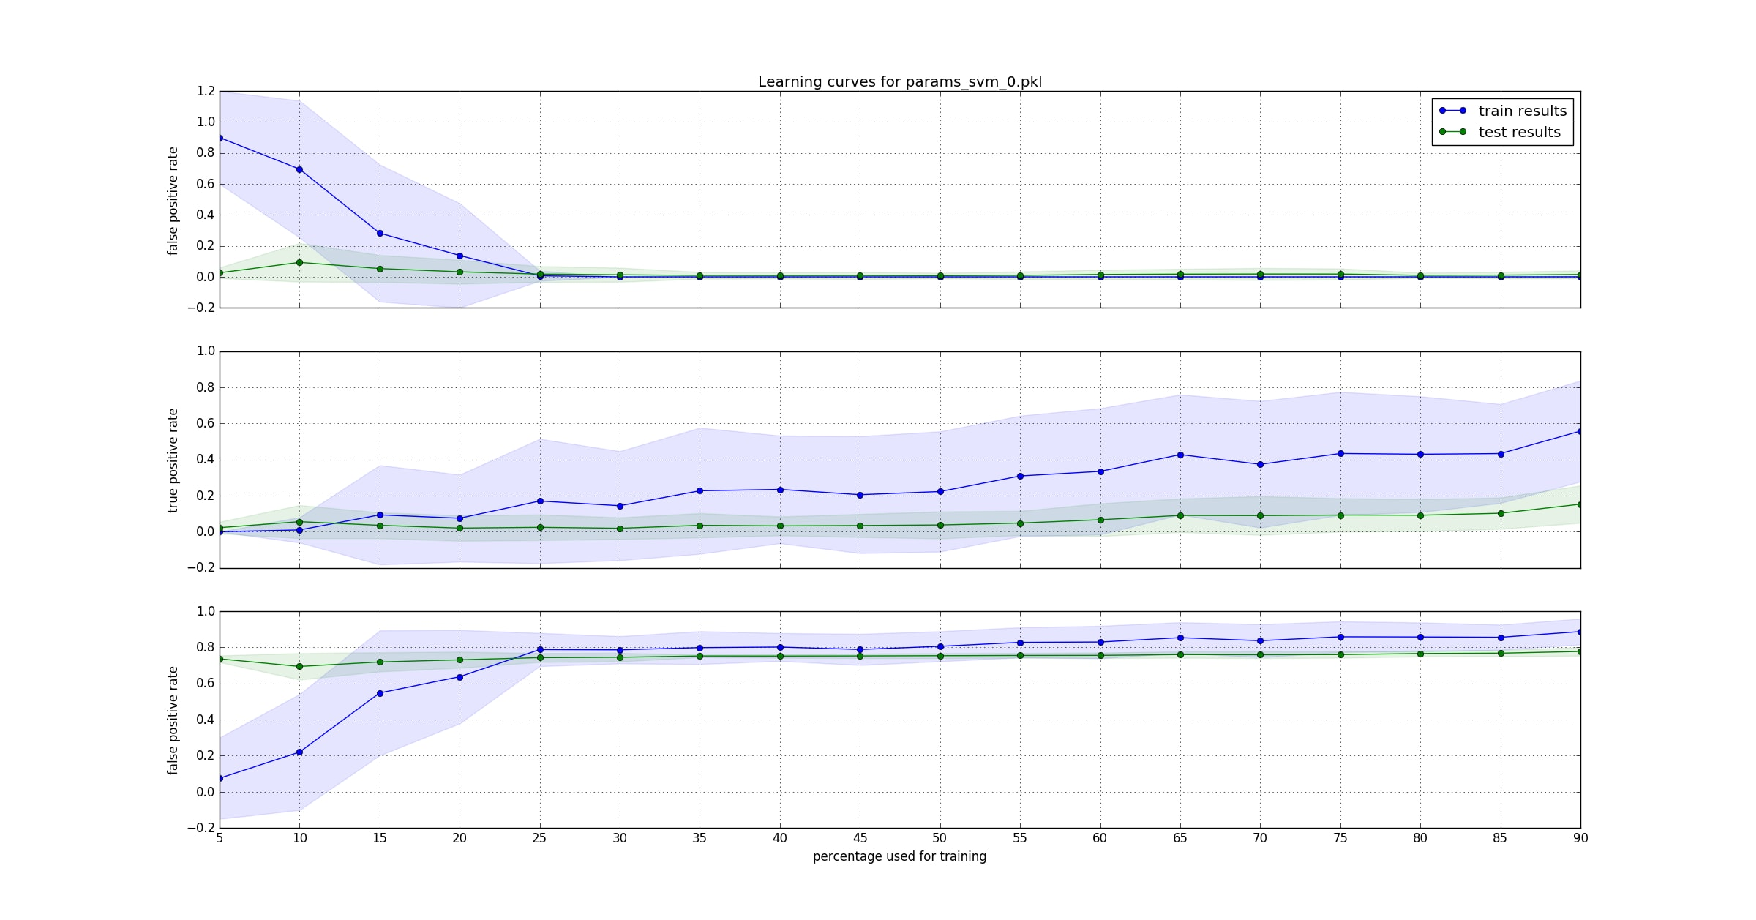
\includegraphics[width=\columnwidth, scale=1]{./Figures/Lc_Ds1_P20-80_SVM}}
\caption{Learning curves, Phase 1, SVM}
\label{learning curves}
\end{center}
\vskip -0.2in
\end{figure} 

\begin{figure}[h]
\vskip 0.2in
\begin{center}
\centerline{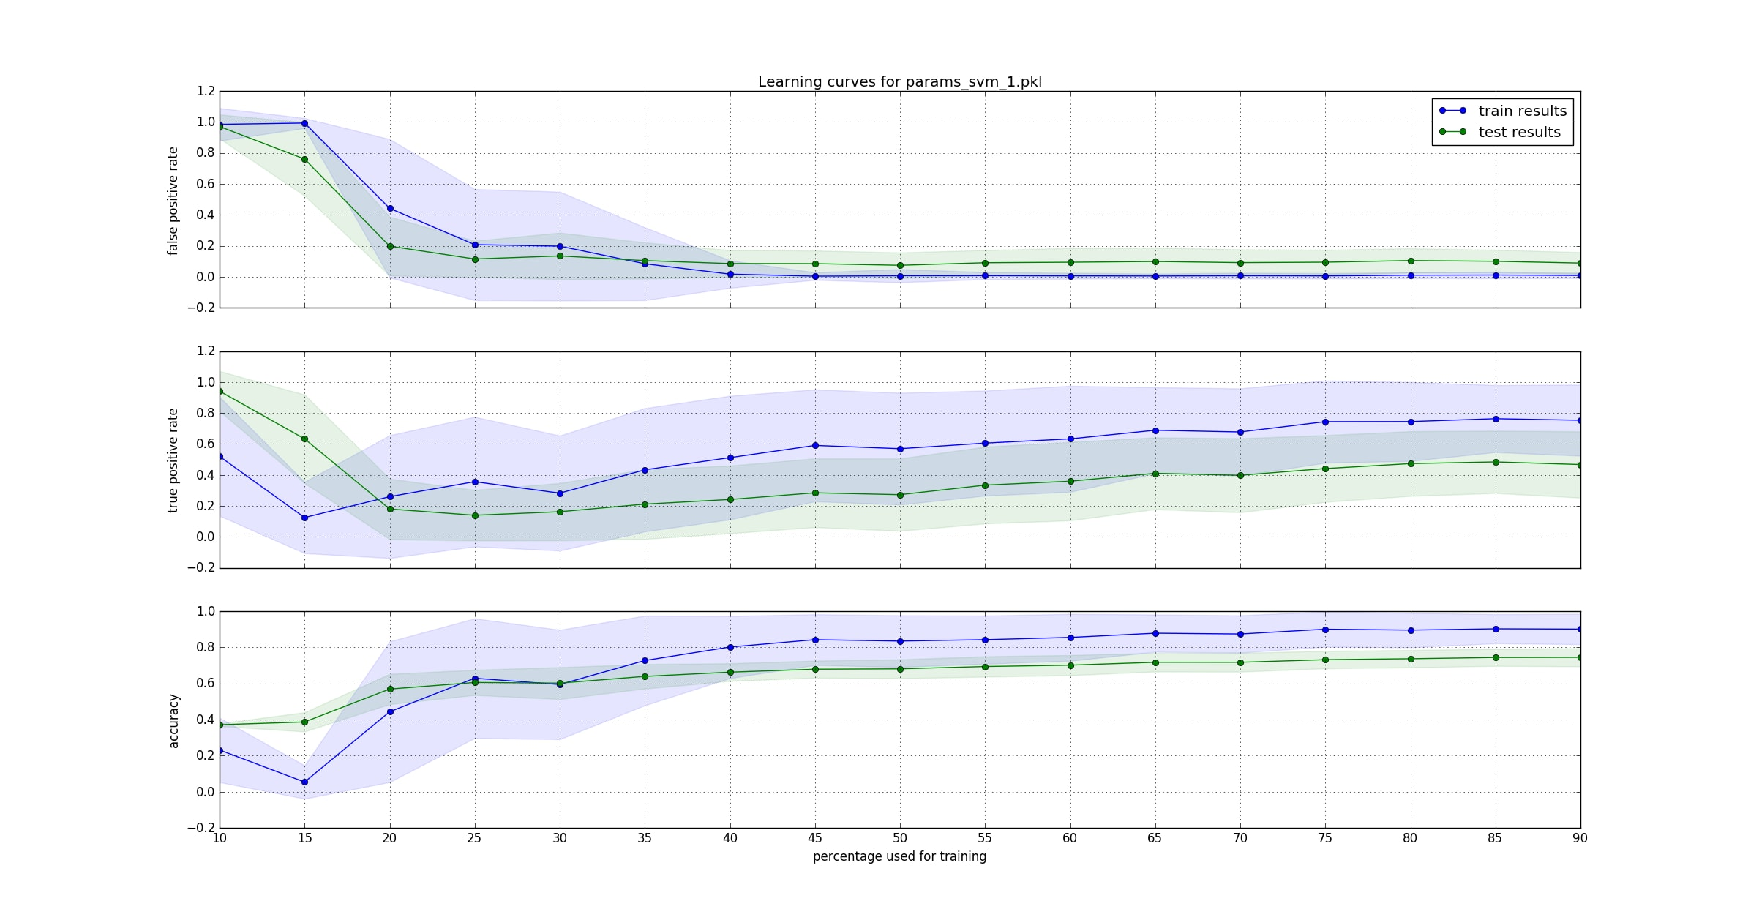
\includegraphics[width=\columnwidth, scale=1]{./Figures/Lc_Ds2_P40-60_SVM}}
\centerline{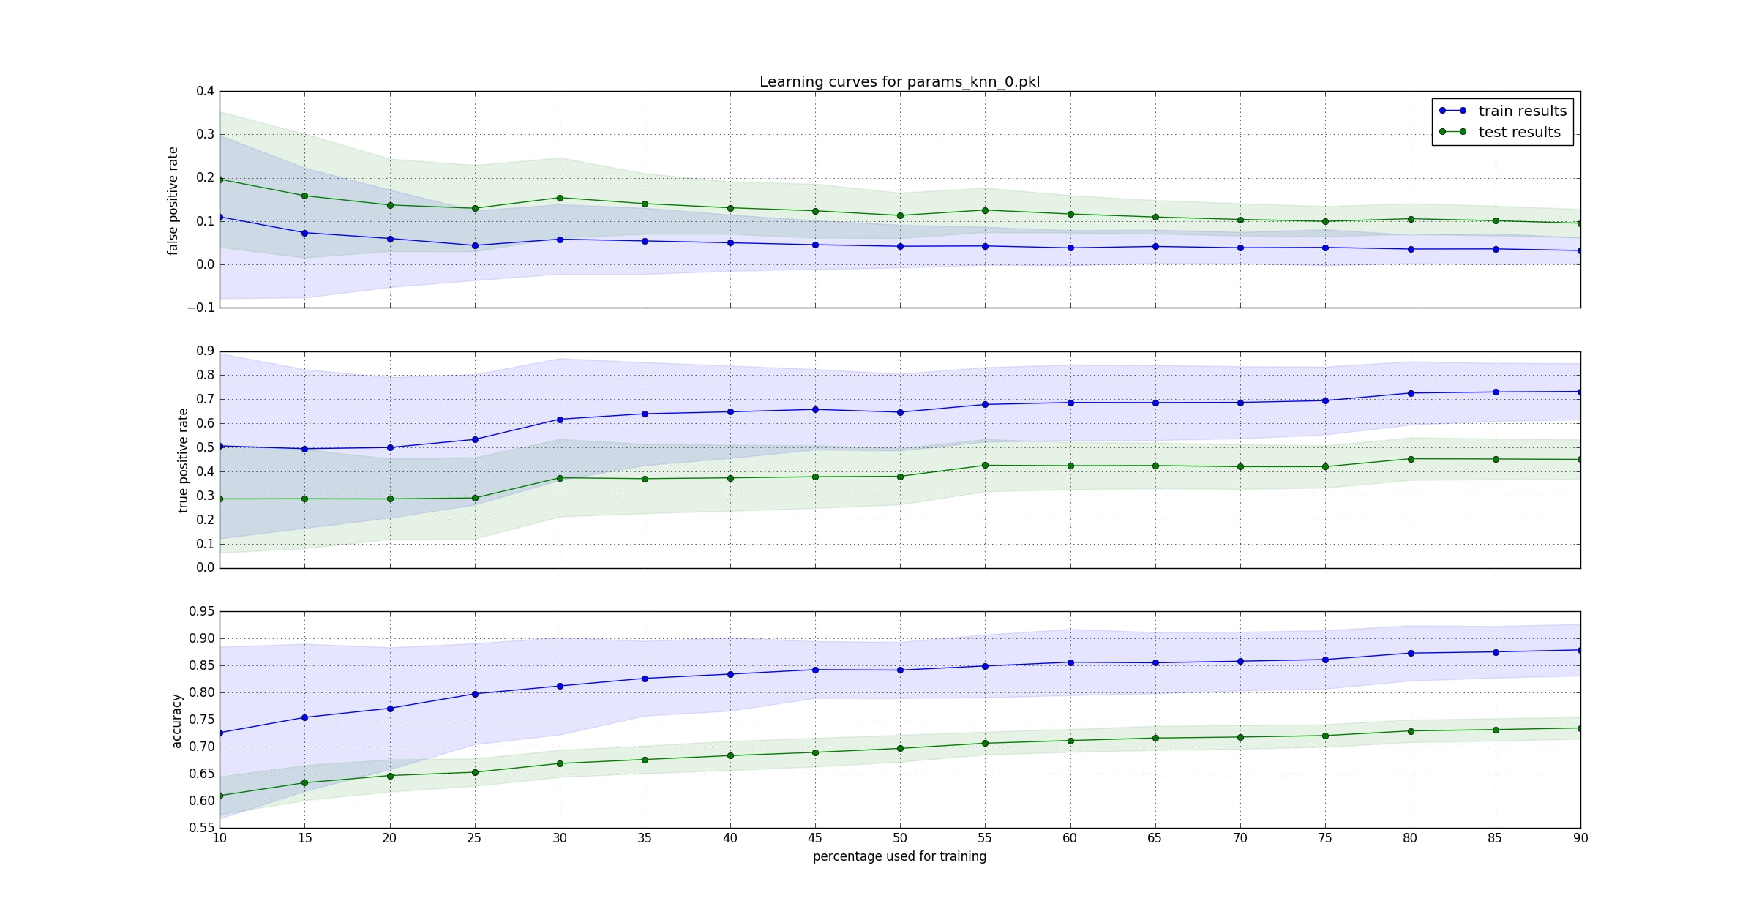
\includegraphics[width=\columnwidth, scale=1]{./Figures/Lc_Ds2_P40-60_kNN}}
\caption{Learning curves, Phase 2, SVM \& and KNN}
\label{learning curves}
\end{center}
\vskip -0.2in
\end{figure} 

\begin{figure}[h]
\vskip 0.2in
\begin{center}
\centerline{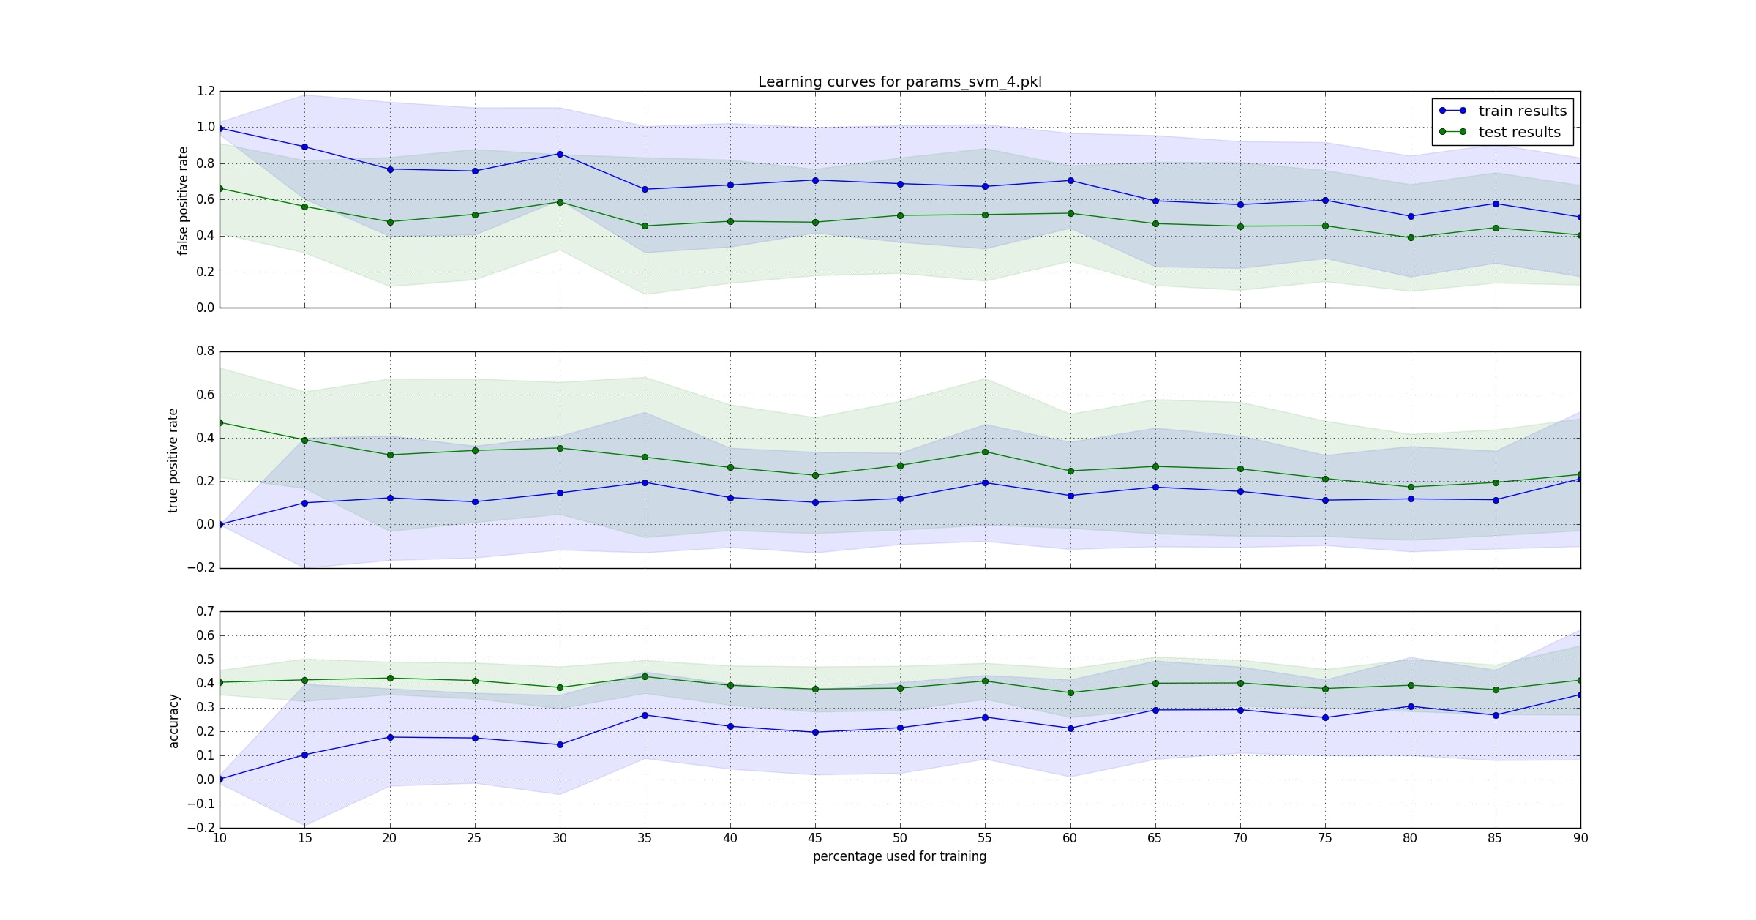
\includegraphics[width=\columnwidth, scale=1]{./Figures/Lc_Ds3_P50-50_SVM}}
\centerline{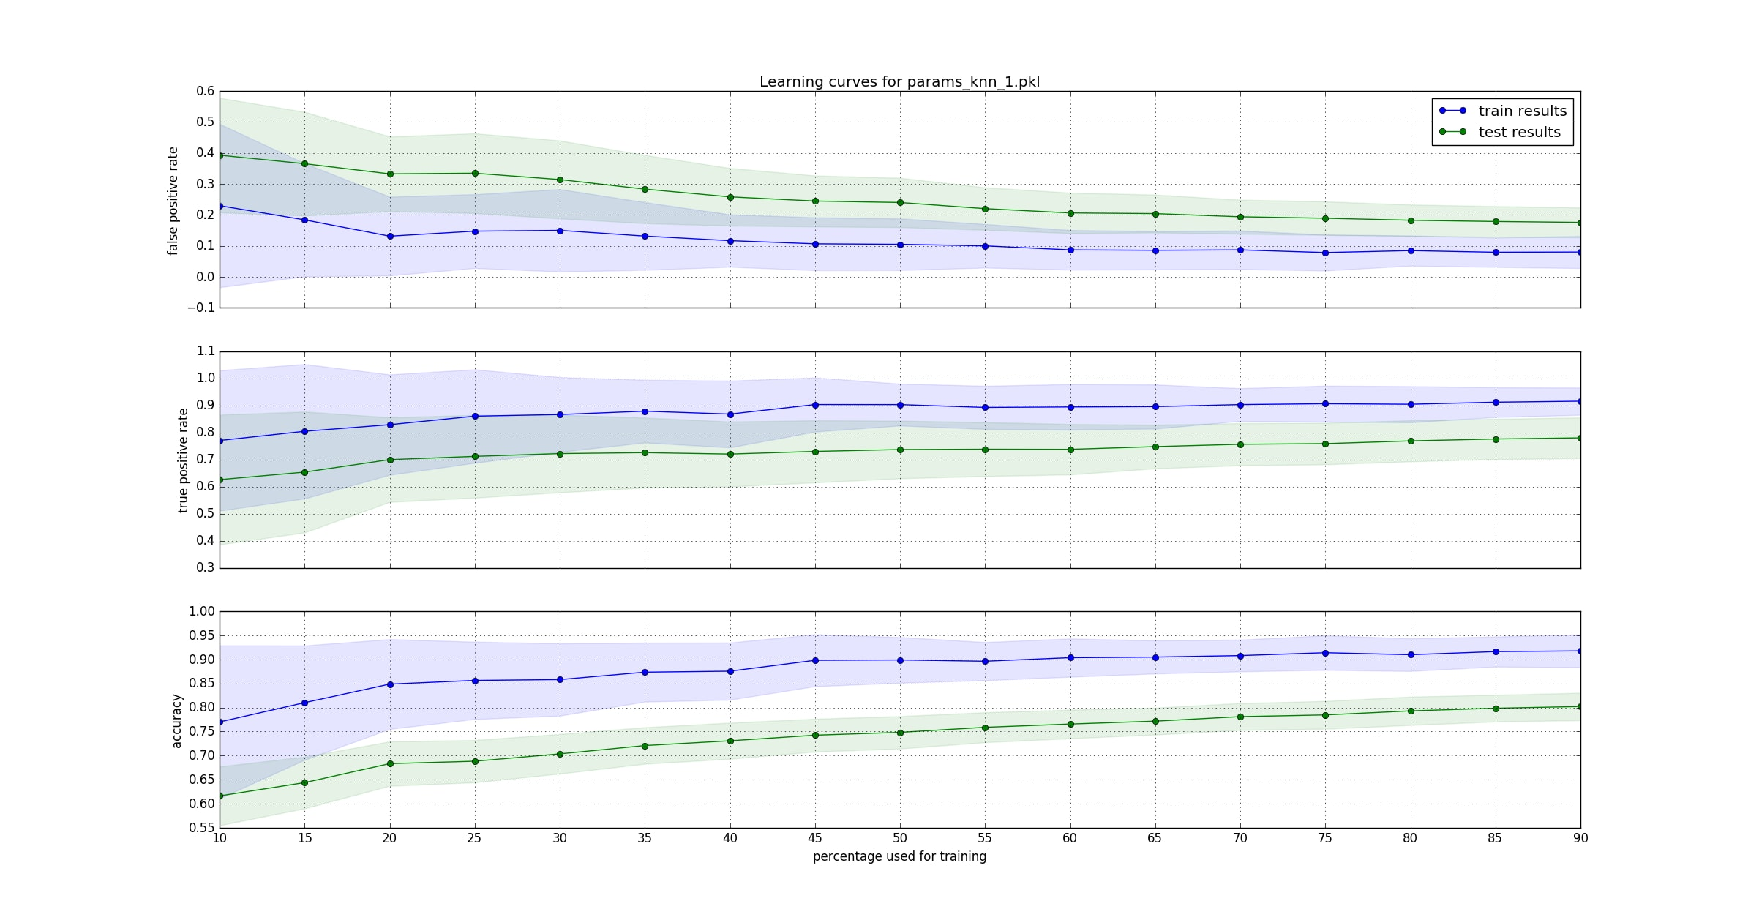
\includegraphics[width=\columnwidth, scale=1]{./Figures/Lc_Ds3_P50-50_kNN}}
\caption{Learning curves, Phase 3, SVM and KNN}
\label{learning curves}
\end{center}
\vskip -0.2in
\end{figure} 

\begin{figure}[h]
\vskip 0.2in
\begin{center}
\centerline{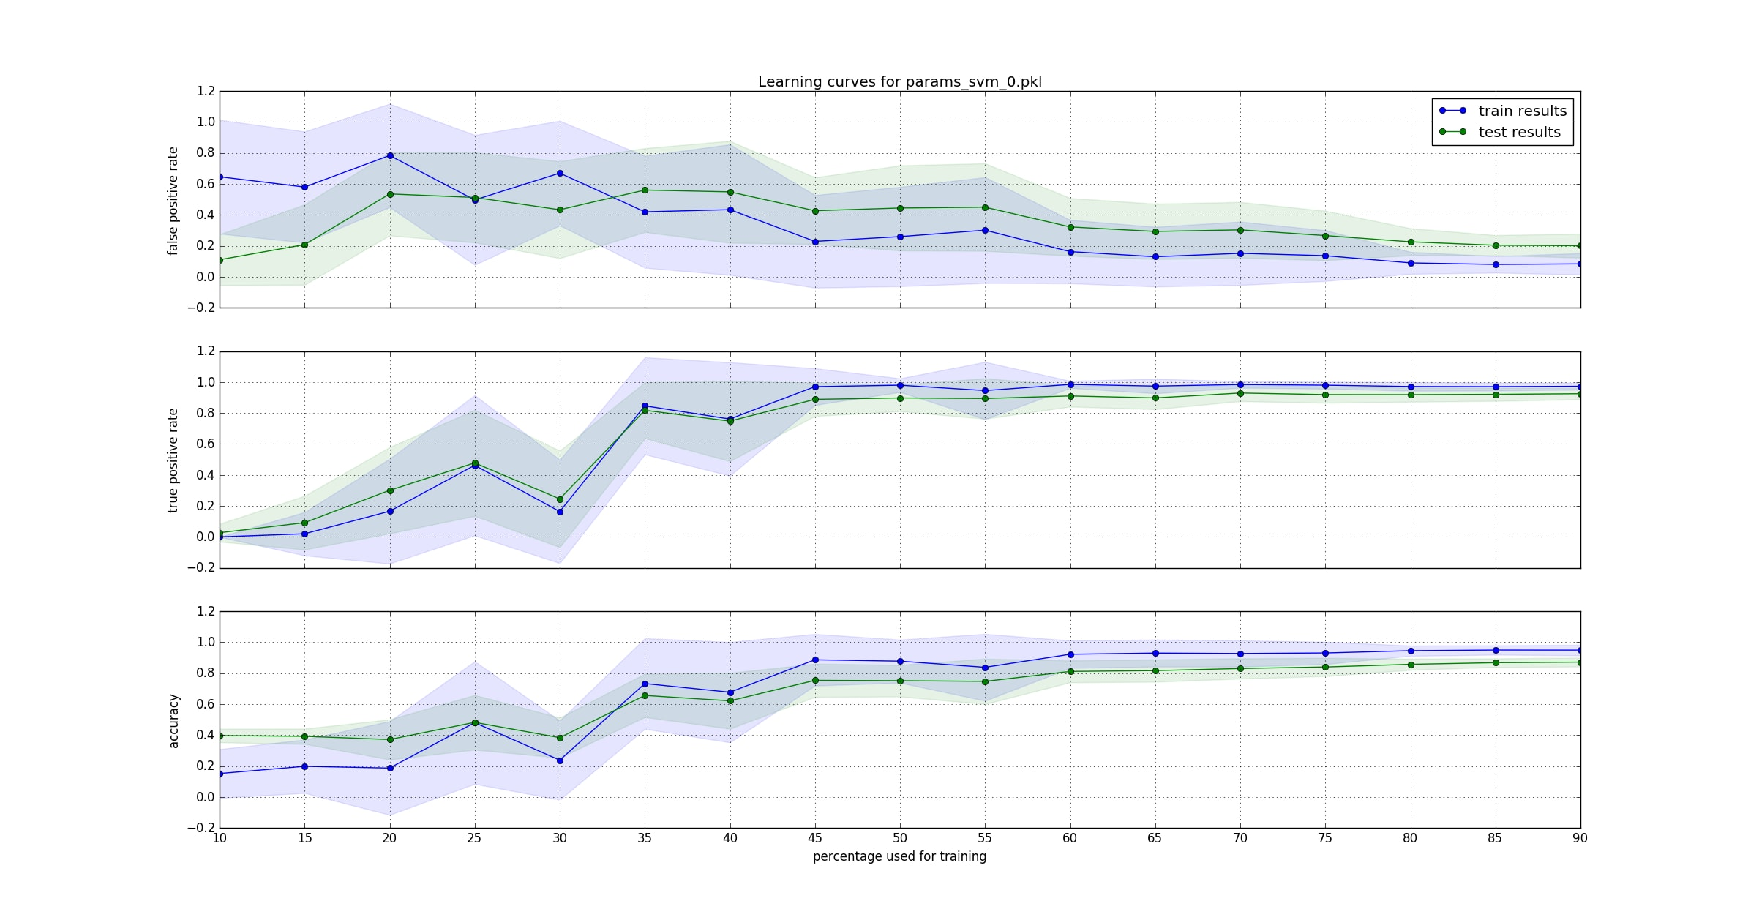
\includegraphics[width=\columnwidth, scale=1]{./Figures/Lc_Ds4_P60-40_SVM}}
\centerline{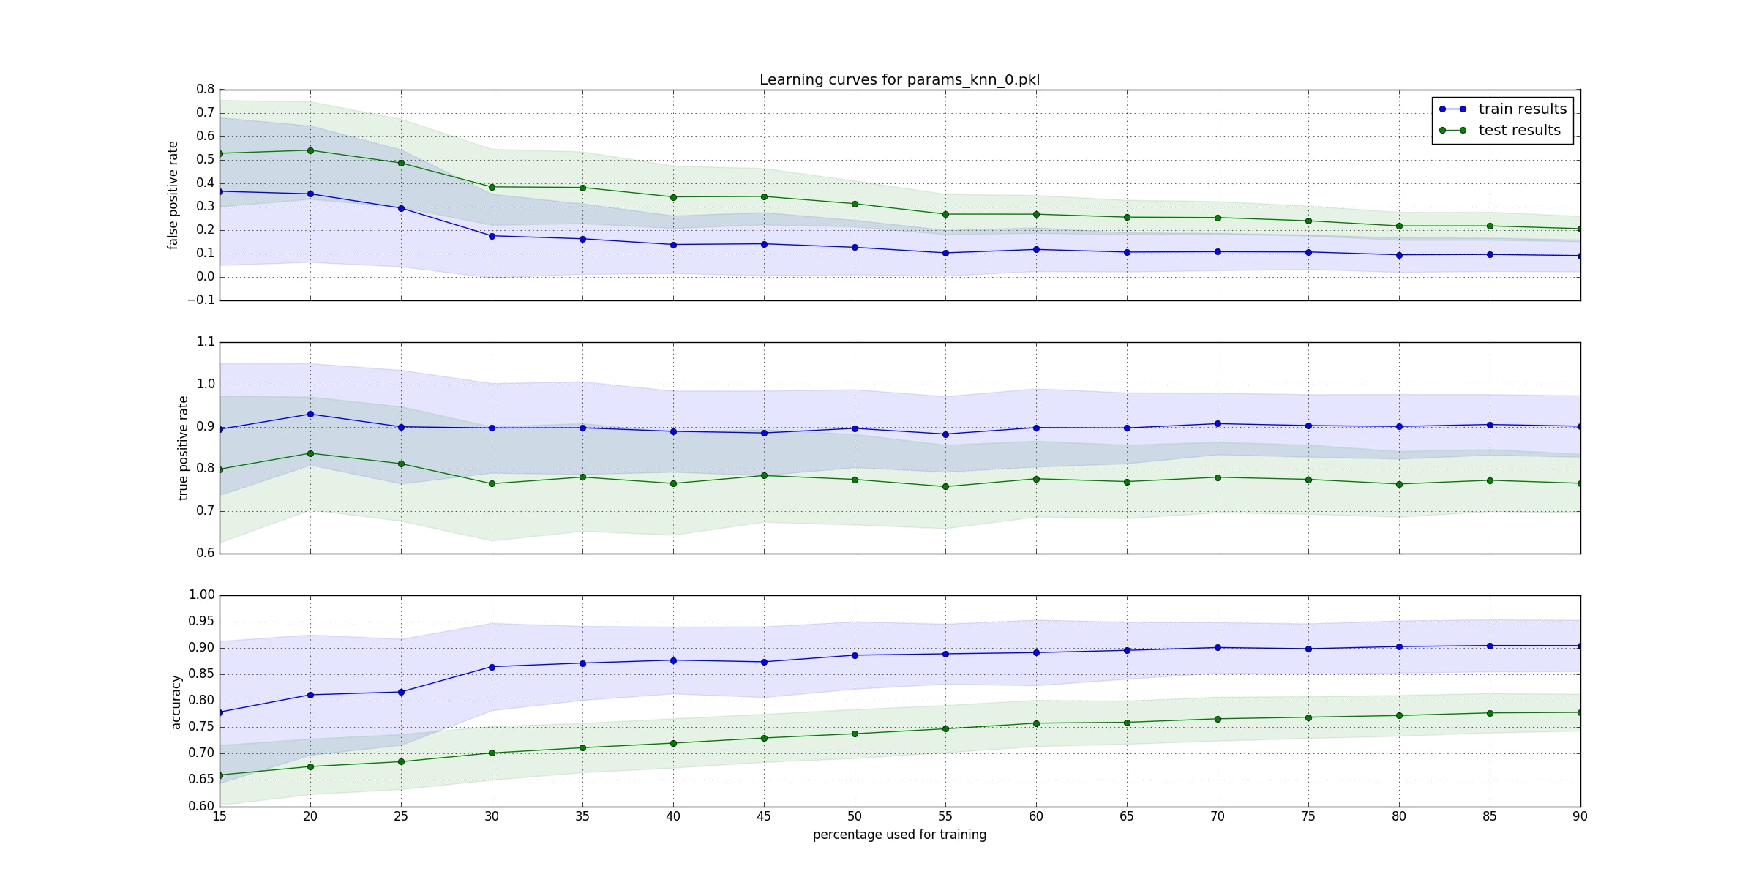
\includegraphics[width=\columnwidth, scale=1]{./Figures/Lc_Ds4_P60-40_kNN}}
\caption{Learning curves, Phase 4, SVM and KNN}
\label{learning curves}
\end{center}
\vskip -0.2in
\end{figure} 


\begin{figure}[h]
\vskip 0.2in
\begin{center}
\centerline{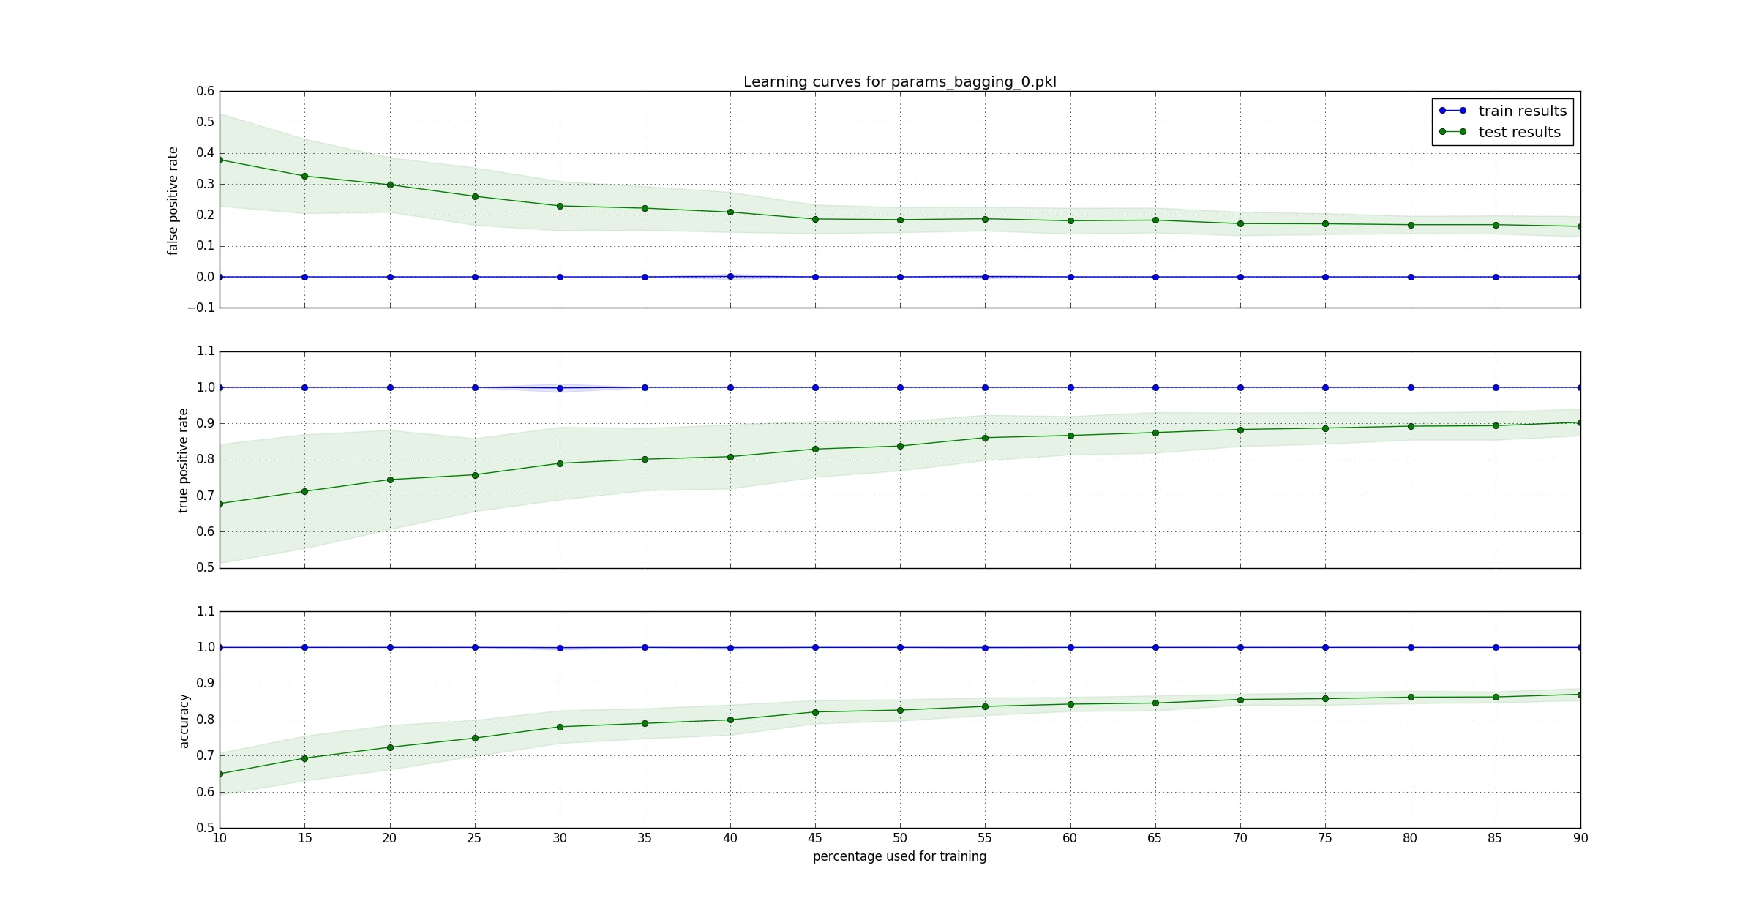
\includegraphics[width=\columnwidth, scale=1]{./Figures/Lc_Ds5_P50-50_BaD}}
\centerline{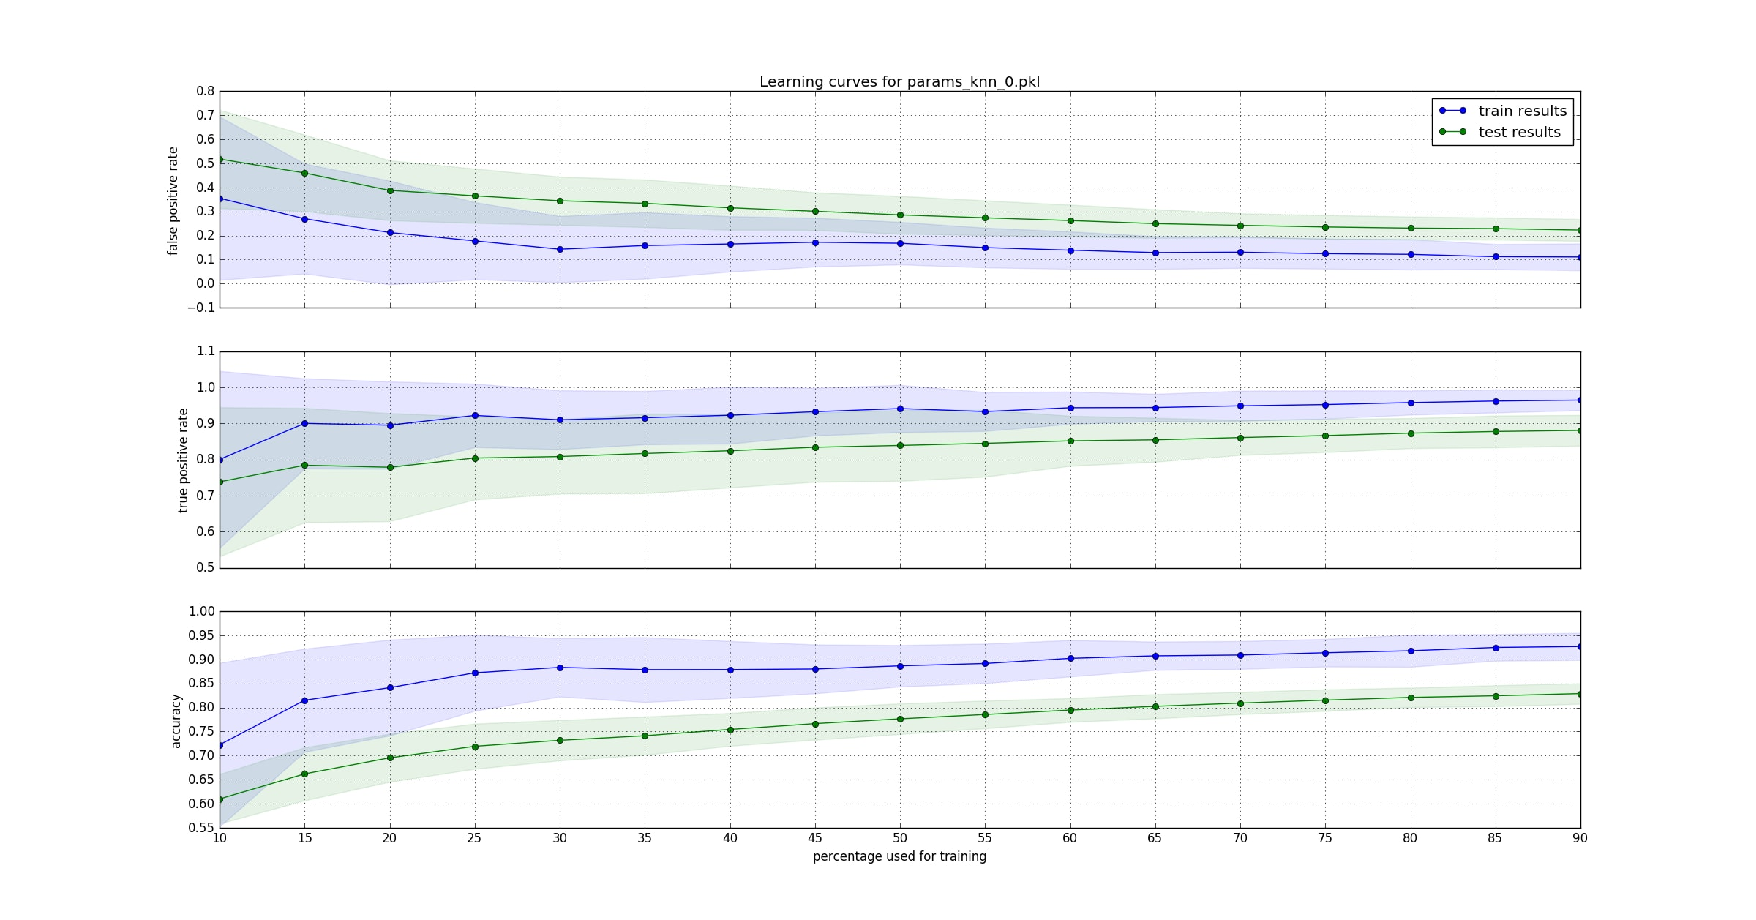
\includegraphics[width=\columnwidth, scale=1]{./Figures/Lc_Ds5_P50-50_Bak}}
\caption{Learning curves, Bagging classifier, Decision Tree, KNN and SVM estimators}
\label{learning curves}
\end{center}
\vskip -0.2in
\end{figure}


\section{Conclusion} \label{Conclusion}

\bibliographystyle{./IEEEtran}
\bibliography{acousticFall}




% that's all folks
\end{document}

